\section{Messaufbau}
In diesem Kapitel befinden sich die verschiedenen Komponenten, welche für den Messaufbau benötigt wurden. Dazu gehören die Spannungsverstärkerschaltung, welcher auf den Arduino montiert ist, das eingebaute Filter sowie der Arduino, welcher für die verschiedenen Funktionen programmiert wurde.
\subsection{Laboraufbau}
Um die Simulationen in die Praxis umzusetzen, wurde ein \grqq T-Drive 3Ph compact Thyristorsteller\grqq \hspace{0.03cm} von der Firma Chemtronic, vom Betreuer zur Verfügung gestellt. Wie der Name des Produktes schon sagt, arbeitet dieser Thyristorschaltung mit 3 Phasen. Für die Ansteuerung des Zündwinkels kann ein Potenziometer verwendet werden, dies hat jedoch den Nachteil, dass der Zündwinkel von Hand eingestellt werden muss. Jedoch kann für die Ansteuerung auch ein Spannungssignal von \SI{0}{V} - \SI{10}{V} benutzt werden. Dieses Spannungsignal entsprich linear dem Zündwinkel 180\textdegree \hspace{0.02cm} bis 0\textdegree \hspace{0.02cm} der Thyristoren. Um dieses Spannungssignal erzeugen zu können, wurde ein Arduino Mega 2560 verwendet. Das Problem dabei ist, dass der Arduino nur eine Ausgangsspannung von \SI{5}{V} erzeugen kann. Deshalb wurde eine Spannungsverstärkungsschaltung designt, welche die Spannung verdoppelt. Um die variable Spannung zu erzeugen, wurde im Arduino die PWM-Funktion genutzt. Diese läuft mit einer Frequenz von \SI{490}{Hz}. Für die Ansteuerung sollte aber eine reine DC-Spannung geliefert werden. Deshalb wurde zusätzlich ein Tiefpass-Filter erster Ordnung am Ausgang des Arduinos eingebaut, mit einer Cut-off Frequenz von \SI{1}{Hz}.  


\subsubsection{Filter}
Um die Elemente des passiven Tiefpassfilters zu berechnen, wurde folgende Formel verwendet.
\begin{equation}
f = \frac{1}{2 \cdot \pi \cdot R_1 \cdot C_1}
\end{equation}
Dabei wurde $f$ = \SI{1}{Hz} eingesetzt und so kann die Kapazität oder der Widerstand frei gewählt werden. Für die Kapazität wurde \SI{10}{\mu F} ausgesucht. Somit ergab sich einen Widerstand von \SI{16}{\Omega}. Die Bauteile wurden aufgrund der vorhandenen Bauteile im Labor ausgewählt.


\subsubsection{Verstärkerschaltung}
Die Verstärkung einer nicht invertierenden Verstärkungsschaltung wird wie folgt berechnet.
\begin{equation}
V_u = 1 + \frac{R_3}{R_2}
\end{equation}
Um die Ströme klein zu halten, wurden Widerstände von \SI{12}{k\Omega} ausgewählt. Um eine Verstärkung von zwei zu erreichen, wurden die beiden Widerstände gleich gross gewählt. 

\newpage
\begin{figure}[ht!]  
	\centering 
	\begin{minipage}[t]{.76\textwidth} \centering 
		\centering
		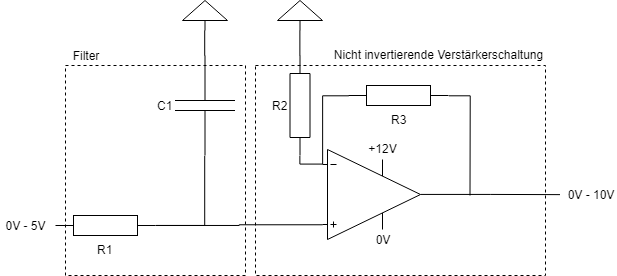
\includegraphics[scale=0.555]{Schema_Verstaerkerschaltung.png}	
		\caption{Schema Verstärkerschaltung}\label{fig:Verstaerkerschaltung}
	\end{minipage}	
	% 
	\begin{minipage}[b]{.23\textwidth}
		\centering
		\begin{tabular}{|l|l|}
			\hline
			R$_1$ & \SI{16}{k\Omega} 	\\ 	\hline
			R$_2$ & \SI{12}{k\Omega} 	\\ 	\hline
			R$_3$ & \SI{12}{k\Omega} 	\\	\hline
			C$_1$ & \SI{10}{\mu F} 		\\	\hline
		\end{tabular}
		\caption{Werte der Bauteile}
		\label{tab:Verstaerkerschaltung}
	\end{minipage}
\end{figure} 



Nach dem Aufbau der Verstärkerschaltung wurde die Ausgangsspannung bei einem Duty-cycle von 1 gemessen. Dabei wurde ein Wert von \SI{9.885}{V} gemessen. Dies bedeutet das der Thyristorsteller nicht voll ausgesteuert werden kann. Deshalb wurde bei der Verstärkerschaltung die Verstärkung erhöht. 

\begin{equation}
\frac{12k\Omega}{11k\Omega} = 1.09
\end{equation}
Dies resultiert in eine Verstärkung von:
\begin{equation}
V_u = 1 + \frac{12k\Omega}{11k\Omega} = 2.09
\end{equation}
Nach dem Einbau des neuen Widerstandes wurde eine Spannung von \SI{10.2}{V} am Ausgang gemessen. Somit steht der ganze Bereich von \SI{0}{V} - \SI{10}{V} zur Verfügung.

\subsection{Laboraufbau mit einem Widerstand}
Nach dem Feststellen der Funktionalität der Spannnungsverstärkungsschaltung, konnte mit dem Laboraufbau begonnen werden. Hierzu wurde ein variabler Culatti-Widerstand als Last benutzt. Dieser hat den Vorteil das die Last bei allen Phasen symetrisch ist. Um den Strom klein zu halten, wurde ein Widerstand von \SI{150}{\Omega} gewählt. Der Aufbau der Messschaltung ist auf der Abbildung \ref{fig:Messaufbau} ersichtlich. 

\begin{figure}[ht!]
	\centering
	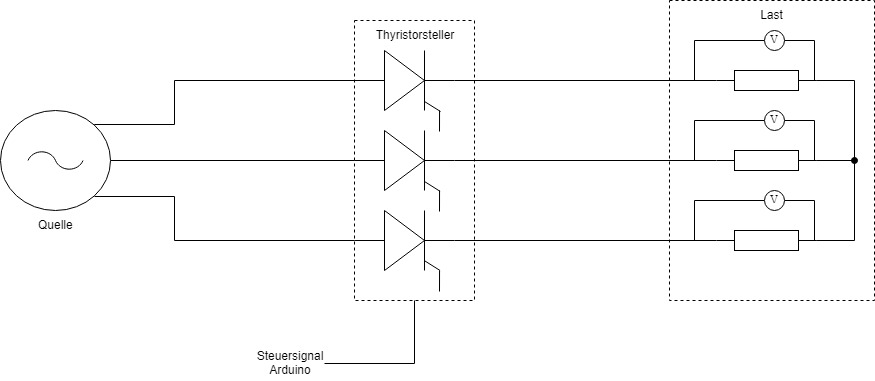
\includegraphics[width=\textwidth]{Messaufbau.png}	
	\caption{Schema Laboraufbau mit einem dreiphasigen Widerstand in Stern}\label{fig:Messaufbau}
\end{figure}

Um zu analysieren wie sich die Spannung bei der Last in Dreieck verläuft, wurde die Last auch in Dreieck geschaltet.

\subsection{Laboraufbau mit einer ASM}
Gleich wie beim Laboraufbau wurde bei diesen Versuchen eine ASM als Motor in den Stromkreis geschaltet. Dabei wurde auch wieder der Motor in Stern und in Dreieck geschaltet. Für die ASM wurde eine kleine Maschine der Marke Lukas Nülle mit einer Leistung von \SI{0.3}{kW} verwendet. Dies hat den Grund, dass bei dieser Maschine ein Drehzahlgeber vorhanden war um die Drehzahlen messen zu können. Da die Maschine nicht wie der Widerstand, eine rein ohmsche Last ist, verhielten sich die Spannungen und Ströme anders. Ein weiterer interessanter Punkt bei dem Motor ist, dass wenn die Spannung abgeschaltet wird, die Motor sich noch ausdrehen muss und so sehr träge auf Veränderungen reagiert.

\subsection{Arduino}
Das Arduino-Programm, welches den Thyristorsteller ansteuert, wurde mit der Arduinosoftware geschrieben. Vorteil des Arduinos ist, dass die Software Open-source ist und sich für fast jede erdenkliche Arbeit auf dem Internet Beispielcodes befinden. Desweitern ist eine grosse Versibilität durch den Arduino gewährleistet. Mit den verschiedenen I/O Pins können Spannungen bis zu \SI{5}{V} gemessen und DC-Spannungen mit einem PWM ausgegeben werden.

\subsubsection{Phasenanschnittssteuerung mit Arduino}
Die Phasenanschnittssteuerung wird der einfachen \SI{0}{V} bis \SI{10}{V} Ansteuerung des Thyristorstellers gemacht. Dabei ist die Ansteuerungskennlinie linear und so ensprechen \SI{5}{V} einem Zündwinkel von 90\textdegree. Diese Ansteuerungsbereich muss nur auf die 0 bis 255 Werte umgerechnet werden, da der analogWrite Bereich des Arduinos so konzipiert ist. Wenn so z.B. ein Winkel von 90\textdegree \hspace{0.02cm} erwünscht ist, muss ein Wert von 127 ausgegeben werden.

\subsubsection{Schwingungspaketsteuerung mit Arduino}
Die Schwingungspaketsteuerung funktioniert mit dem Thyristorsteller nicht so einfach, da dieser für Phasenanschnitt konzipiert ist. Jedoch kann beim Arduino zwischen HIGH und LOW umgeschaltet werden, mit einer bestimmten Zeitverzögerung dazwischen. Das Problem was sich dabei stellt, ist dass der Thyristorsteller und die Spannungsverstärkerschaltung beide zusammen eine Zeitverzögerung von \SI{0.2}{s} haben. So schaltet der Sinus verzögern ein und dies resultiert in einem Hochfahren von \SI{0.35}{s}. So verhält sich die Schwingungspaketsteuerung mehr wie ein Auf- und Absteuern.

\subsubsection{Hartes Auf- und Absteuern}
Um das harte Auf- und Absteuern zu implementieren, wurden die beiden vorherigen Verfahren kombiniert. Anstatt jedoch nur einen Winkel vorzugeben, wurde mit einer for-Schleife die Ansteuerungsspannung und somit der Zündwinkel linear erhöht. Sobald sich die Spannung auf dem Maximum befindet, wird für \SI{0.2}{s} gewartet. So wird für eine kurze Zeit die maximale Spannung ausgegeben. Danach wird mit einer zweiten for-Schleife runtergefahren. Die Geschwindigkeit des Hoch- \& Runterfahrens kann verändert werden. Die Auswirkungen der Geschwindigkeit der Steigung wird im Kapitel \todo{Kapitel mit Steigung} genauer erklärt. Wenn die minimale Spannung erreicht ist, wird \SI{0.1}{s} gewartet bis das nächste Hochfahren anfängt, dies hat den Grund da sonst das Spannungssignal nicht auf Null geht. Diese zwei for-Schleifen befindet sich in einer driten for-Schleife. Diese ist dafür zuständig, mittels Schwingungspaketsteuerung einstellen zu können wie oft Hoch- \& Runtergefahren wird bevor der ganze Zyklus wieder von vorne beginnt. Wenn z.B. fünf Auf- und Absteuernpakete von zehn durchgeschaltet werden, bedeutet dies, dass fünfmal Hoch- \& Runtergefahren wird und danach werden die nächsten fünf Pakete gesperrt.

\subsubsection{Sanftes Auf- und Absteuern}
Für das sanfte Auf- und Absteuern wird wie der Name schon sagt, langsamer als bei dem harten Auf- und Absteuern hoch- und runtergefahren. Zusätzlich wird nach dem Erreichen der maximalen Spannung eine Verzögerung von \SI{6}{s} eingebaut, bis das Programm wieder runterfährt. Des weiteren bleibt man nach dem Erreichen der minimalen Spannung für \SI{3}{s} auf \SI{0}{V}. Danach fährt das Programm wieder hoch. Dies entspricht auch einem Auf- und Absteuern aber wie im Kapitel \todo{Kapitel mit Steigung} erklärt, verhaltet sich das FFT in diesem Fall ganz anders als mit dem hartem Auf- und Absteuern.

\subsubsection{Drehzahlmessung für eine Reglerauslegung}
Um die Drehzahl der ASM messen und regeln zu können, wurde eine Drehzahlregelung eingebaut. Dabei wird die Spannung über dem Drehzahlgeber gemessen. Die Spannung beträgt bei der maximalen Drehzahl von \SI{2800}{U/min}, \SI{58.8}{V}. Die Spannung ist linear von der Drehzahl abhängig, und beträgt so bei z.B. \SI{1400}{U/min}, \SI{29.4}{V}. Da diese Spannung zu hoch ist um mit dem Arduino messen zu können, muss ein Spannungsteiler eingebaut werden, um die Spannung auf \SI{5}{V} zu reduzieren. 

\begin{equation}
4.94 V = 58.8 V \cdot \frac{56k\Omega}{56k\Omega + 611k\Omega}
\end{equation}

Somit kann die Spannung mit dem Arduino gemessen werden. Dabei wird die Spannung mit dem ADC in 1024 verschiedenen Stufen gemessen. So enspricht der Wert 512 einer Spannung von \SI{2.5}{V}.
\todo{Einfügen Quelle für Spannungsmessung} Zusätzlich wird dieser Wert mit den Widerstandswerten des Spannungsteiler auf die Orginalspannung zurück gerechnet. Für den Regler wird für den Sollwert ein Spannungswert vorgegeben. Damit wird von dem Sollwert der Istwert abgezogen, um die Differenz zu erhalten, welche für den Regler von grosser Bedeutung ist. Da der Ausgabewert des Arduinos einem Wert zwischen 0 und 255 entspricht, muss die Differenz umgerechnet werden. Zusätzlich zur Differenz, wird ein PI-Regler benötigt. 
Mit der Formel: \cite{Quelle_Marco} 
\begin{equation}
Y(k) = Y(k-1)+ B_0U(k)+B_1U(k-1)
\end{equation}
Wobei $Y$ der Ausgangsspannung, $U$ der Differenzspannung und $k$ dem Laufparameter ensprechen \cite{PI_Regler}. Die Parameter $B_0$ und $B_1$ werden folgendermassen berechnet:
\begin{equation}\label{eq:B0}
B_0 = \left(K_p + \frac{K_iT}{2}\right) 
\end{equation}
\begin{equation}\label{eq:B1}
B_1 = -\left(K_p - \frac{K_iT}{2}\right) 
\end{equation}

Nachdem dies berechnet ist, muss die Spannungsdifferenz von der Ausgangsspannung subtrahiert werden. Das Resultat der Berechnung wird wieder in die 0 bis 255 Werte umgerechnet um mit dem analogWrite ausgegeben werden zu können. Die Werte der Ausgangsspannung und der Differenzspannung werden nach der Ausgabe in den Laufparameter $k-1$ geladen. Das Problem mit dem PI-Regler ist, dass der Thyristorsteller und die Spannungsverstärkung eine Totzeit besitzen. Dadurch ist das Auslegen eines guten Reglers nicht möglich. Durch das Gespräch mit anderen Studenten, wurde festgestellt das ein Smithprädiktor \cite{Regelungstechnik_Buch} Abhilfe verschaffen könnte. Dieser rechnet die Totzeiten in das System und dieses kann so genauer geregelt werden. Jedoch wurde der Smithprädikator nicht mehr implementiert. Der Code für die Drehzahlregelung befindet sich im Anhang. \todo{Kapitel angeben}

\begin{figure}[ht!]
	\centering
	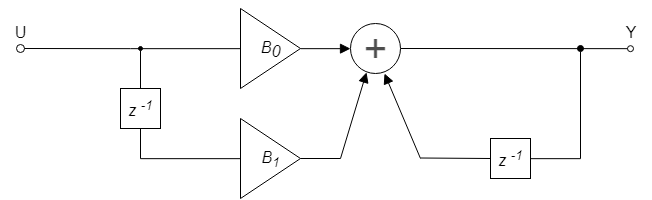
\includegraphics[width=\textwidth]{BlockdiagrammPI.png}	
	\caption{Blockdiagramm eines digitalen PI-Reglers}\label{fig:PIRegler}\cite{PI_Regler}
\end{figure}







